\chapter{Marco Tecnológico}
\label{capitulo3}
\lhead{Capítulo 3. \emph{Marco Tecnológico}}

En este capítulo se mencionan las herramientas utilizadas para el desarrollo
del proyecto de pasantía. Dichas herramientas son descritas brevemente y se menciona
su uso dentro de la solución planteada.

\section{Java}

Java es un lenguaje de programación de propósito general, concurrente, basado en clases
y orientado a objetos. Está diseñado para ser lo suficientemente sencillo para
que muchos programadores puedan alcanzar fluidez en el lenguaje. (\cite{JAVA})

\section{OSGI}

OSGI (\emph{(Open Service Gateway Initiative)}) es un conjunto de especificaciones
que definen un sistema dinámico formado por componentes
para Java. Estas especificaciones permiten un modelo de desarrollo donde las aplicaciones
son dinámicamente compuestas por muchos componentes reutilizables (\cite{OSGI}).

En la figura \ref{layers} se describe el modelo por capas definido por OSGI:

\begin{figure}[h!]
\centering
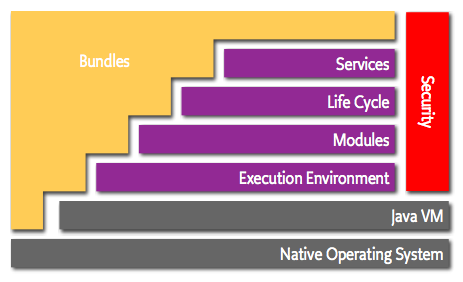
\includegraphics[width=0.4\textwidth]{layering-osgi}
\caption[Capas de OSGI]{Modelo por capas definido en OSGI. (\cite{OSGI})}
\label{layers}
\end{figure}

La siguiente lista contiene una breve descripción de los términos:
\begin{itemize}
\item \textbf{Bundles}: los Bundles son los componentes de OSGI hechos por los desarrolladores.
\item \textbf{Servicios}: la capa de servicios conecta bundles de una manera dinámica intercambiando objectos Java.
\item \textbf{Ciclo de vida}: el API para instalar, arrancar, detener, actualizar y desinstalar un bundle.
\item \textbf{Módulos}: la capa que define como un bundle puede importar y exportar código.
\item \textbf{Seguridad}: la capa que determina los aspectos de seguridad.
\item \textbf{Ambiente de Ejecución}: define que métodos y clases están disponibles en una plataforma específica.
\end{itemize}


\section{Apache Felix}

Apache Felix es un esfuerzo de la comunidad Apache para implementar la especificación de
la plataforma OSGI bajo la licencia Apache. La especificación OSGI es ideal para
cualquier proyecto interesado en los principios de modularidad, desarrollo orientado
a componentes y desarrollo orientado a servicios (\cite{FELIX}).

\section{JDBC}

El \emph{API} JDBC (\emph{Java Database Connectivity}) es el estándar en la industria
para conectividad independiente del manejador de base de datos entre programas escritos en
Java y una gran variedad de bases de datos (\cite{JDBC}). Para cada uno de los manejadores
de base de datos que se desean conectar a través de un programa Java deberá existir una implementación
del estándar JDBC, también llamado Driver, que le permite al programa comunicarse a través del
API con el manejador de base de datos.

\section{Base de datos Oracle}

La base de datos Oracle es un sistema de manejo de base de datos relacional (\cite{ORACLE})
producido y mantenido por Oracle Corporation.

\section{PostgreSQL}

PostgreSQL es un poderoso sistema de bases de datos relacional. Tiene más de
15 años de desarrollo activo y una arquitectura que se ha ganado la reputación de tener
integridad de datos, confiabilidad y correctitud de datos (\cite{POSTGRE}).

\section{Microsoft SQL Server}
Microsoft SQL Server es un sistema de manejo de bases de datos relacional desarrollado por
Microsoft.

\section{Arquitectura ePhoenix}

Construido sobre la base de Apache Felix, la arquitectura ePhoenix le brinda a los
equipos de desarrollo del BBVA todas las herramientas necesarias para desarrollar programas
que realicen procesamiento por lotes o publiquen servicios web.

Abarcar todas las funcionalidades que ofrece la arquitectura escapa del alcance del
proyecto de pasantías, por lo que se trabajará con los componentes de ePhoenix
que se encargan de realizar las conexiones a bases de datos usando JDBC.

\section{HTML}

HTML, que significa Lenguaje de Marcado para Hipertextos (HyperText Markup Language)
es el elemento de construcción más básico de una página web y se usa para crear y
representar visualmente una página web. Determina el contenido de la página web,
pero no su funcionalidad (\cite{HTML}).

\section{Javascript}

JavaScript es un lenguaje ligero e interpretado, orientado a objetos, más conocido
como el lenguaje de script para páginas web. Es un lenguaje script multi-paradigma, dinámico,
soporta estilos de programación funcional, orientada a objetos e imperativa (\cite{JS}).

\section{Node.js}
Node.js es un entorno de ejecución para JavaScript construido con el motor de JavaScript V8
de Chrome. Node.js usa un modelo de operaciones de entrada y salida sin bloqueo y orientado a eventos.
El ecosistema de paquetes de Node.js, npm, es el ecosistema mas grande de librerías
de código abierto en el mundo (\cite{NODE}).

\section{JSON}
JSON (\emph{JavaScript Object Notation}) es un formato de intercambio de datos ligero.
Esta diseñado para ser fácil de leer y escribir por humanos y fácil de parsear y generar
por las máquinas (\cite{JSON}).

\section{Angular}
Angular es una plataforma escrita en JavaScript que facilita el proceso
de crear aplicaciones para la web. Angular combina plantillas declarativas, inyección de dependencias
y buenas prácticas integradas para solucionar problemas a la hora de desarrollar (\cite{ANGULAR}).
Además, al presentar una arquitectura que combina el desarrollo orientado a componentes
y el patrón de diseño MVC, Angular ofrece grandes ventajas en cuanto a mantenibilidad
y reusabilidad de código.

\section{Arquitectura Thin2}

Para la arquitectura Thin2 se tomó como base el framework de aplicaciones web Angular. Partiendo
de la capacidad de Angular de definir componentes reutilizables se le ofrecen a los
equipos de desarrollo varios elementos predefinidos para realizar las tareas más
comunes a la hora de escribir una página web. Entre estos componentes se pueden
mencionar el componente para obtener configuraciones de un servidor o el que implementa
la autenticación y autorización propia manejada dentro de BBVA.

\section{Herramientas para la gestión del proyecto}

Aparte de las tecnologías utilizadas para desarrollar el proyecto se utilizaron
las siguientes herramientas para la gestión de la pasantía y el control de versiones:

\subsection{Dimensions CM}

Dimensions CM is un gestor de cambios y configuraciones que disminuye eficientemente
la complejidad del desarrollo paralelo, integrando y automatizando prácticas de desarrollo
(\cite{DIMENSIONS}).

Dimensions CM es la herramienta utilizada en el BBVA para el control de versiones, control de
calidad y el despliegue de aplicaciones.

\subsection{Jira}

Jira Software es una herramienta de gestión de proyectos para equipos ágiles (\cite{JIRA}).
Entre sus características ofrece una manera sencilla de manejar y visualizar
las tareas asignadas mediante la metodología de trabajo SCRUM.
